%
%
\pgfplotsset{colormap={rdoryl}{
rgb(0)=(1, 1, 0.80000000000000004)
rgb(1)=(1, 0.96678200000000003, 0.71879999999999999)
rgb(2)=(1, 0.93134899999999998, 0.63218799999999997)
rgb(3)=(0.998139, 0.89219499999999996, 0.54929600000000001)
rgb(4)=(0.99617100000000003, 0.85282599999999997, 0.46662100000000001)
rgb(5)=(0.99607800000000002, 0.77780899999999997, 0.38394499999999998)
rgb(6)=(0.99607800000000002, 0.70103800000000005, 0.30126900000000001)
rgb(7)=(0.99418700000000004, 0.62805100000000003, 0.26777400000000001)
rgb(8)=(0.99221800000000004, 0.55521699999999996, 0.23627799999999999)
rgb(9)=(0.99024999999999996, 0.43280299999999999, 0.20096900000000001)
rgb(10)=(0.98828099999999997, 0.30878899999999998, 0.16553599999999999)
rgb(11)=(0.94017700000000004, 0.20592099999999999, 0.137793)
rgb(12)=(0.89096500000000001, 0.10356, 0.110235)
rgb(13)=(0.81656300000000004, 0.051580000000000001, 0.12918099999999999)
rgb(14)=(0.741761, 0.00040000000000000002, 0.148866)
rgb(15)=(0.62203799999999998, 0, 0.14902000000000001)
rgb(16)=(0.50196099999999999, 0, 0.14902000000000001)
}}
% 
\begin{tikzpicture}[scale=\figurewidth]
    \tikzstyle{image} = [inner sep=0, outer sep=0, node distance = 0 and 0]
    % \pgfplotsset{colormap={warm}{
    rgb=(1, 1, 1)
    rgb=(0.98823499999999997, 0.98039200000000004, 0.87058800000000003)
    rgb=(0.99215699999999996, 0.96470599999999995, 0.71372500000000005)
    rgb=(0.98823499999999997, 0.95686300000000002, 0.64313699999999996)
    rgb=(0.98039200000000004, 0.91764699999999999, 0.50980400000000003)
    rgb=(0.96862700000000002, 0.87451000000000001, 0.40784300000000001)
    rgb=(0.94901999999999997, 0.82352899999999996, 0.32156899999999999)
    rgb=(0.92941200000000002, 0.77647100000000002, 0.27843099999999998)
    rgb=(0.90980399999999995, 0.71764700000000003, 0.235294)
    rgb=(0.89019599999999999, 0.65882399999999997, 0.196078)
    rgb=(0.87843099999999996, 0.61960800000000005, 0.168627)
    rgb=(0.87058800000000003, 0.54901999999999995, 0.156863)
    rgb=(0.85097999999999996, 0.47450999999999999, 0.145098)
    rgb=(0.83137300000000003, 0.41176499999999999, 0.13333300000000001)
    rgb=(0.81176499999999996, 0.34509800000000002, 0.11372500000000001)
    rgb=(0.78823500000000002, 0.26666699999999999, 0.094117599999999996)
    rgb=(0.74117599999999995, 0.18431400000000001, 0.074509800000000001)
    rgb=(0.69019600000000003, 0.12548999999999999, 0.062745099999999998)
    rgb=(0.61960800000000005, 0.062745099999999998, 0.043137300000000003)
    rgb=(0.54901999999999995, 0.027451, 0.070588200000000004)
    rgb=(0.47058800000000001, 0.0156863, 0.090196100000000001)
    rgb=(0.40000000000000002, 0.0039215700000000001, 0.101961)
    rgb=(0.34902, 0, 0.129412)
}}

    \node[image] (image1)
    {
        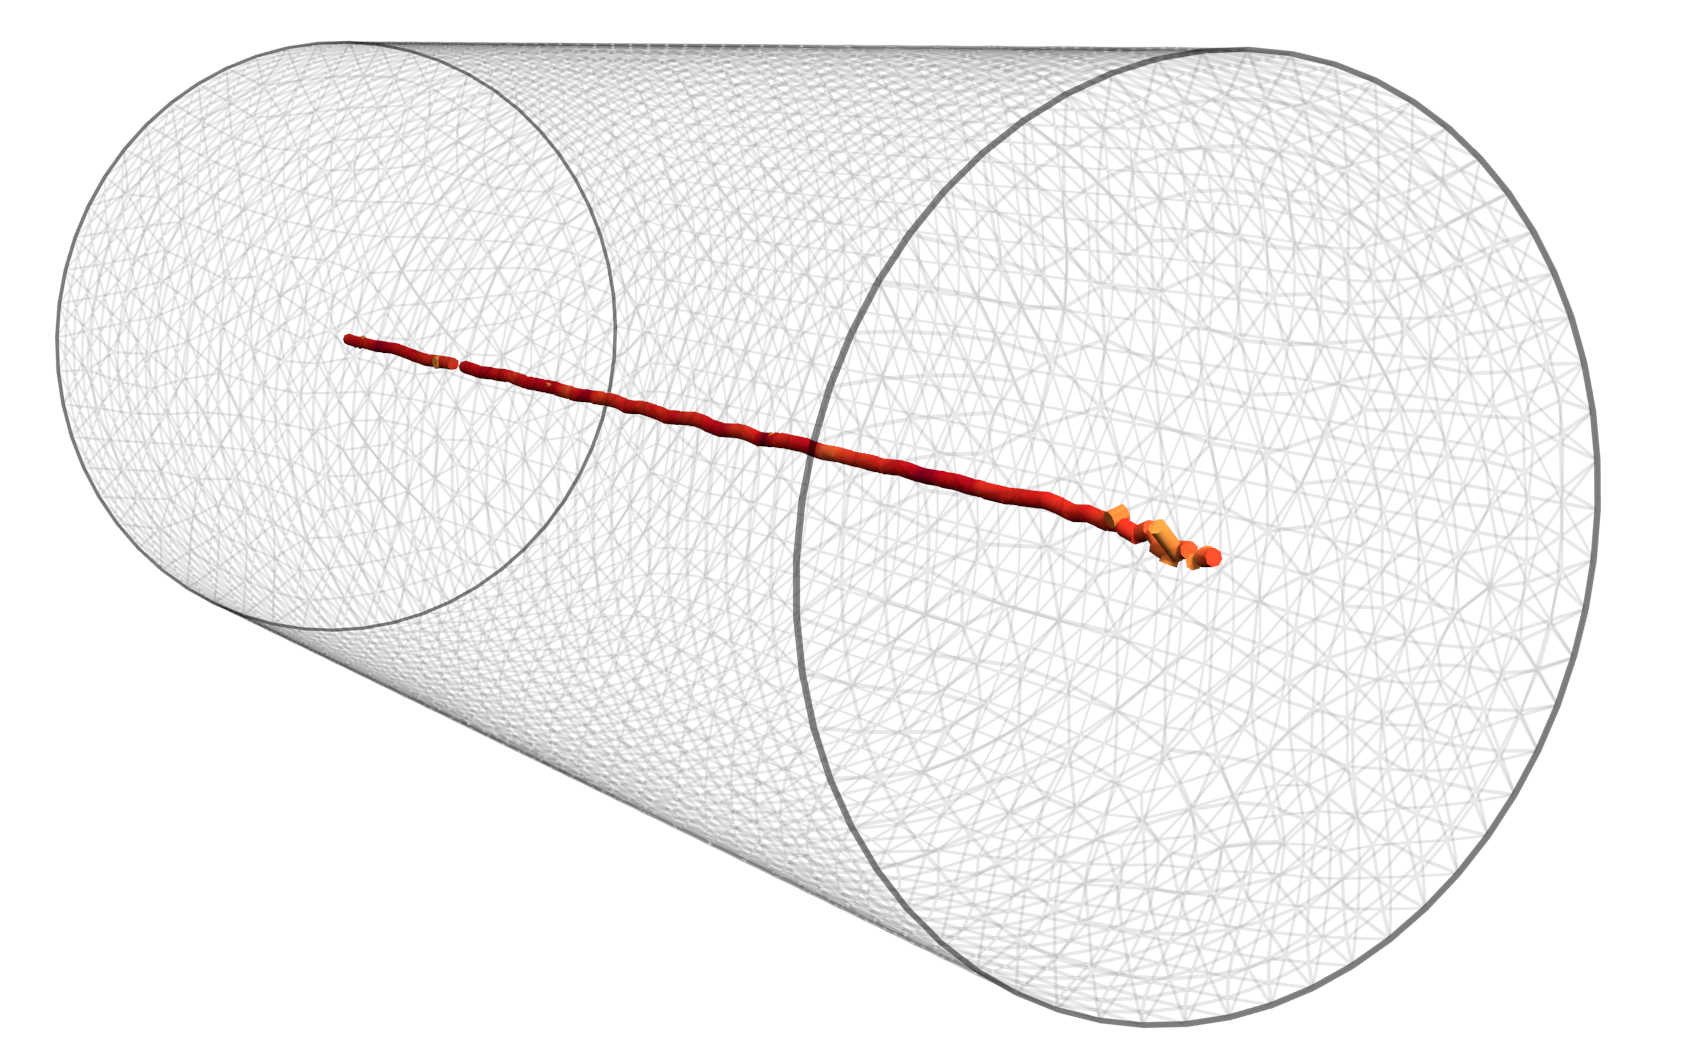
\includegraphics[width=0.45\figurewidth]{figures/cylinder_lines_m100}%
    };
    \node[anchor=south west] at (image1.south west) {\small $M = \num{100}$};

    \node[image, right=of image1] (image2)
    {
        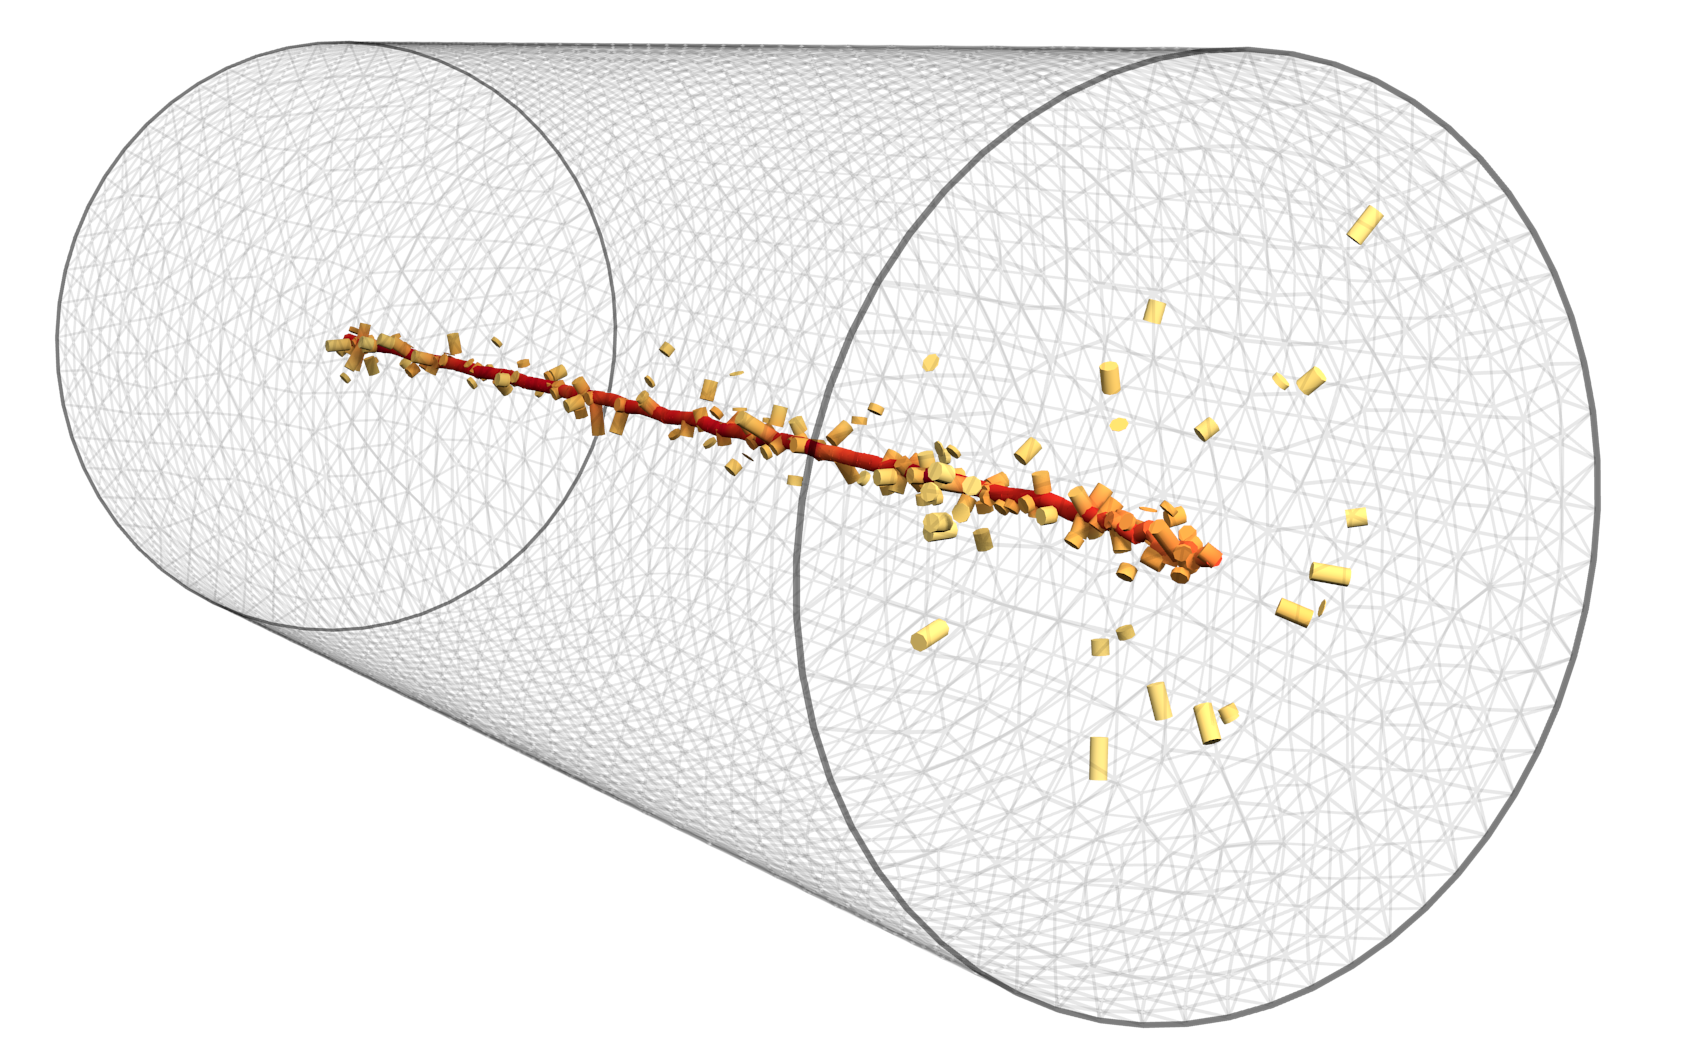
\includegraphics[width=0.45\figurewidth]{figures/cylinder_lines_m1000}%
    };
    \node[anchor=south west] at (image2.south west) {\small $M = \num{1000}$};

    \node[image, below=of image1, yshift=-0.1cm] (image3)
    {
        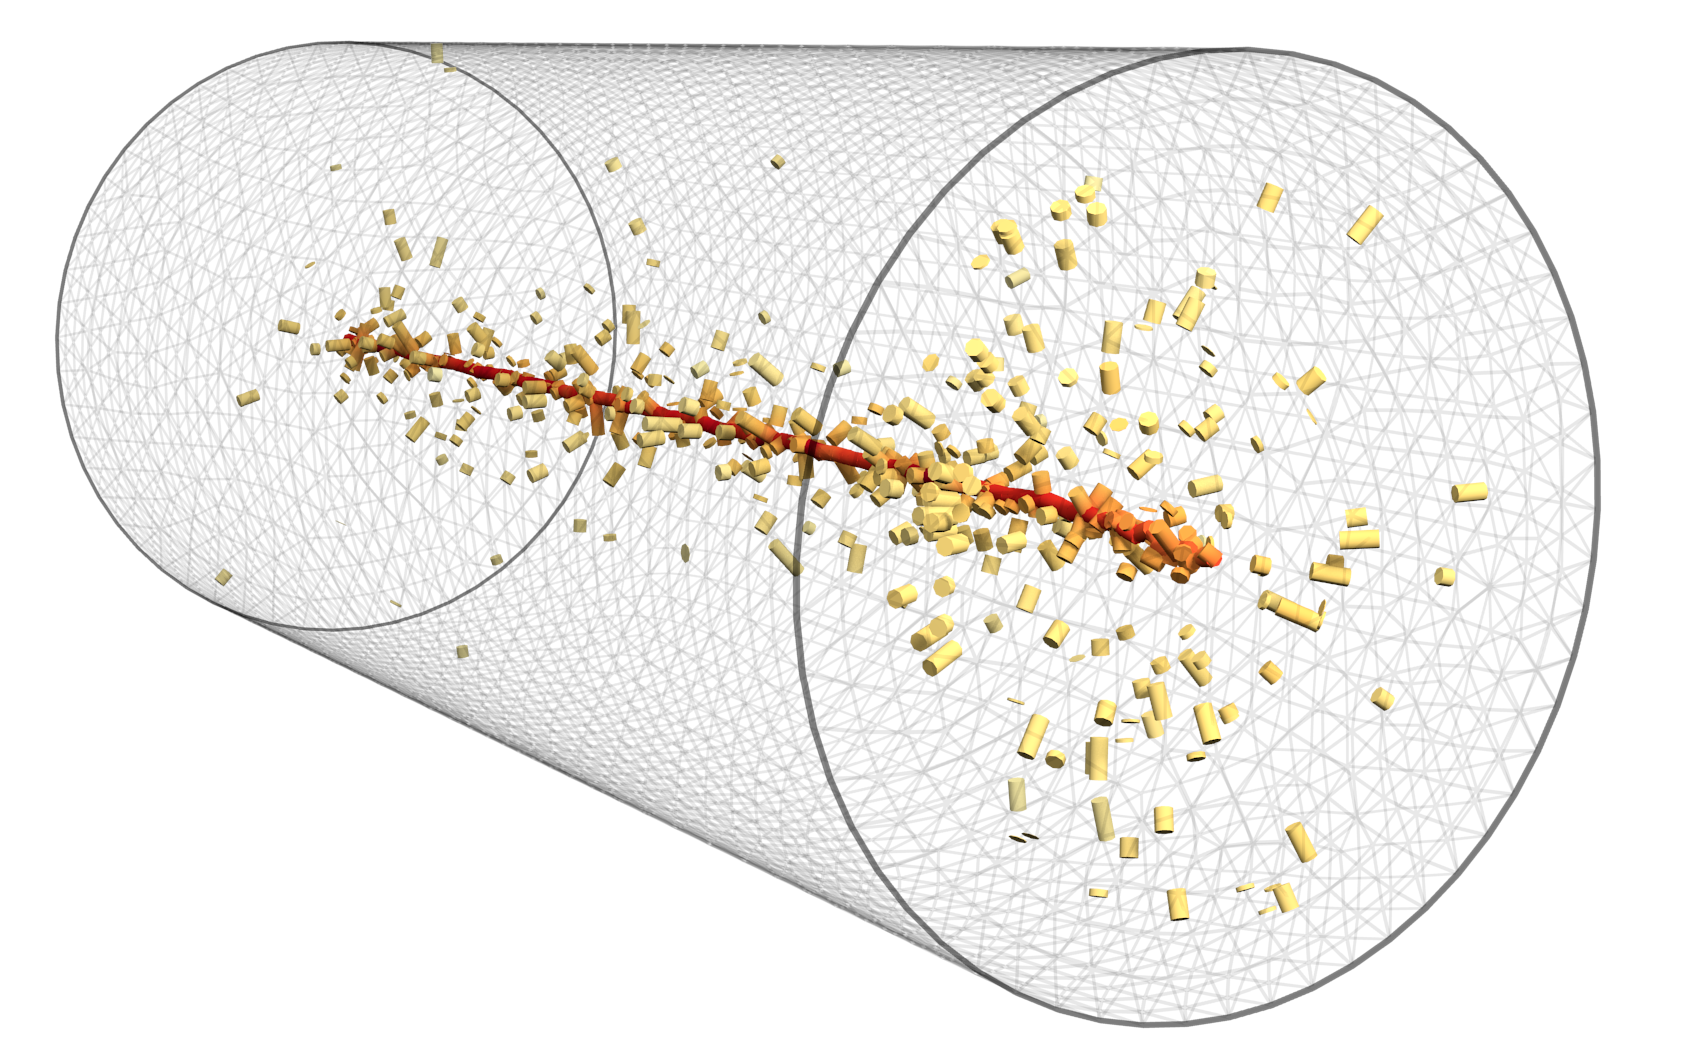
\includegraphics[width=0.45\figurewidth]{figures/cylinder_lines_m10000}%
    };
    \node[anchor=south west] at (image3.south west) {\small $M = \num{10000}$};

    \node[image, right=of image3] (image4)
    {
        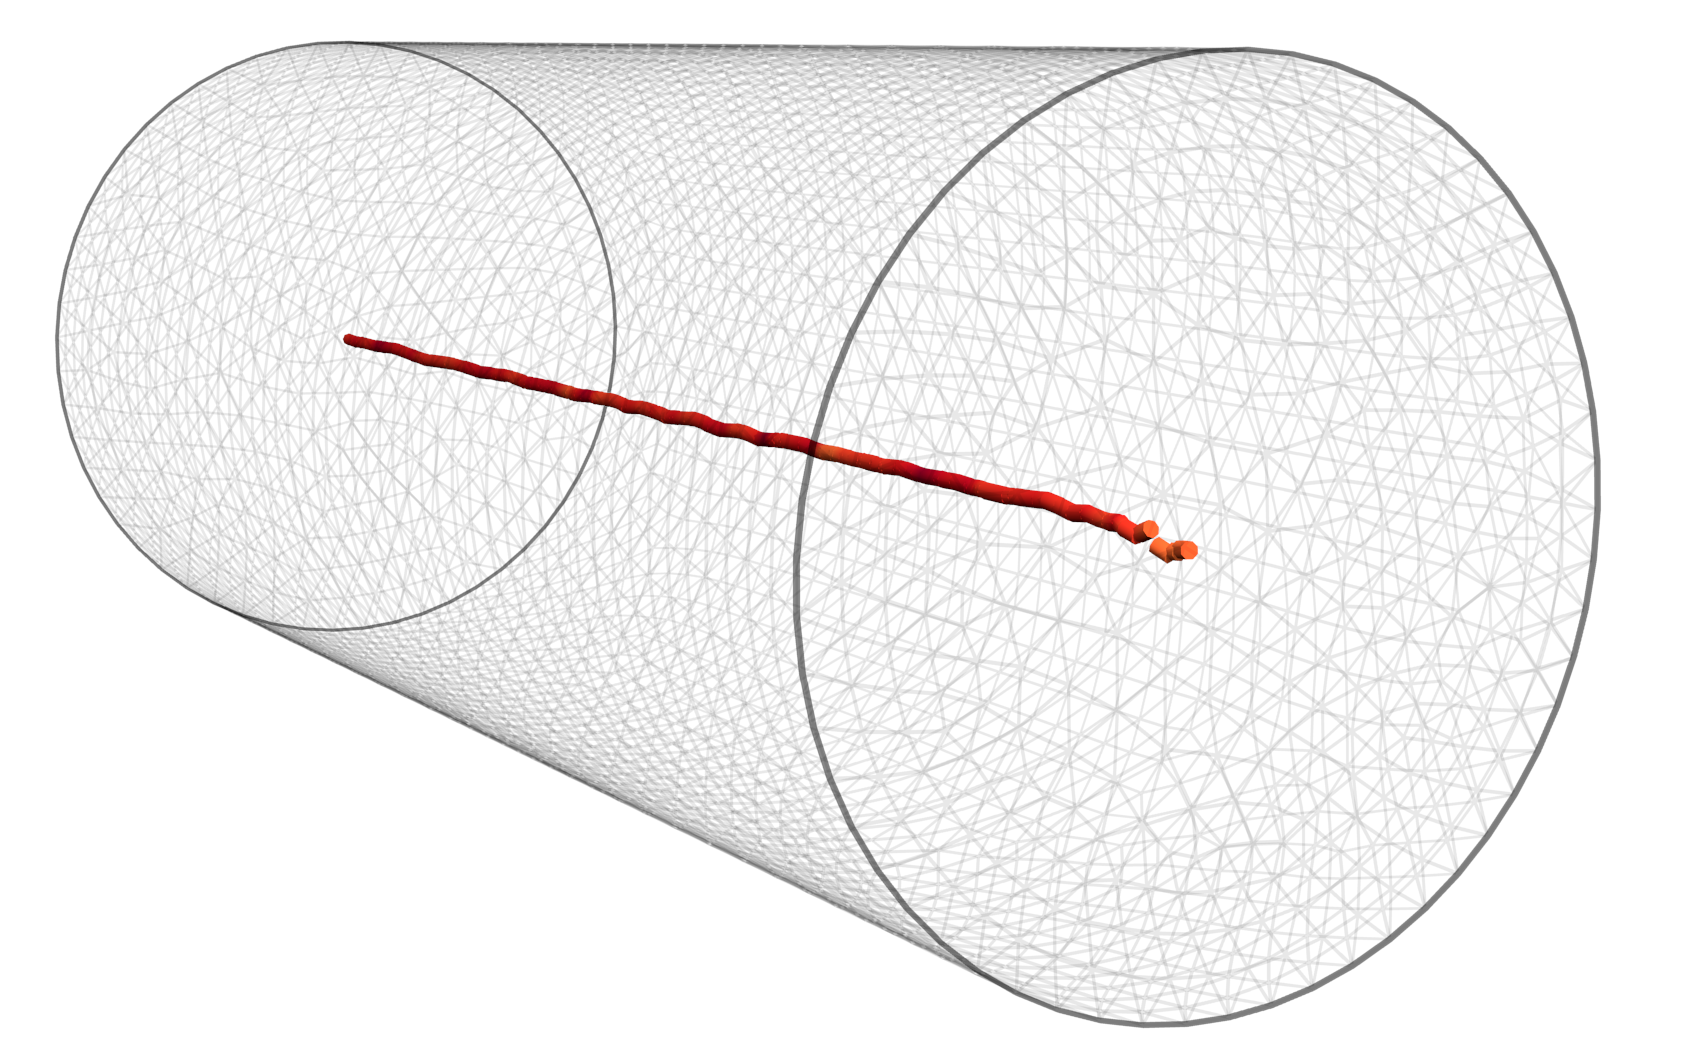
\includegraphics[width=0.45\figurewidth]{figures/cylinder_lines_filtered}%
    };
    \node[anchor=south west] at (image4.south west) {\small filtered};

    \node[anchor=west, xshift=-0.75cm] at (image4.north east){
        \begin{axis}[
        scale only axis,
        height=4cm,
        hide axis,
        domain=1:20,
        colorbar,
        colorbar/width=0.25cm,
        colormap name={rdoryl},
        point meta min=1, point meta max=20,
        colorbar style={
            title=$\log(s)$,
            scaled ticks=false,
            ytick={1, 20}
        }]
      \end{axis}
    };

\end{tikzpicture}